% !TeX root = ../../../main.tex

Starting from the concerns exposed in the previous section, the need for some
changes in the methodology became manifest.
%
There is no clear indication that all of the possible issues enumerated might
be solved keep using a \nn, but especially there is no special need not to
consider any other alternative.

One of the points was if there is a way to determine the distribution, rather
than the individual elements of the samples, one by one.
%
Following this path, one can start considering having a \nn that fits a batch
of replicas together, but how many?
%
All replicas share the same theory, through the \fktab{}s (cf.\
\cref{ch:pine}), that already limits the resources required, but fitting the
whole set at the same time is prohibitive.
%
Moreover, there was the need of a more direct and insightful approach.
%
Taking mainly into account these two points, an alternative solution start
looking promising: why not to directly apply \textbf{Bayesian inference} to the
\pdf posterior determination?

Bayesian inference is sufficiently well-known, and already applied in a series
of contexts, including \hep theory (e.g.\ see \cite{Cacciari:2011ze}, as
described in \cref{ch:mhou}).
%
The basic essence lies in the so-called Bayes theorem:
\begin{equation}
  P(A|B) = \frac{P(B|A) P(A)}{P(B)}
  \label{eq:gp/bayes}
\end{equation}

In the context of inference, the Bayes theorem is usually written:
\begin{equation}
  P\left(\theta|\{x\}\right) = \frac{P\left(\{x\}|\theta\right) P\left(\theta\right)}{
    \int \dd\theta~ P\left(\{x\}|\theta\right) P\left(\theta\right)
  }
  \label{eq:gp/bayes-inf}
\end{equation}
Differences in the notation are minimal, and the integration in the denominator
essentially correspond to $P(\{x\})$.
%
But the interpretation is fundamental:
\begin{description}
  \item[data] $\{x\}$ is a set of observations
  \item[parameter] $\theta$ is an unknown parameter, that enters the
    distribution of the observations, and can thus be inferred from them
  \item[prior] $P(\theta)$ is the prior knowledge about the parameter $\theta$
    (also \enquote{the \textit{prior}}), before any observation is considered
  \item[likelihood] $P\left(\{x\}|\theta\right)$ is the likelihood of the data
    observed, given the value of the parameter $\theta$
  \item[posterior] $P\left(\theta|\{x\}\right)$ is the probability distribution
    of the parameter $\theta$, after the observations $\{x\}$ are taken into
    account
  \item[evidence] is the normalization of the right-hand side, i.e.\ the
    denominator
\end{description}

So, even before the experiment is performed, the observer has a prior knowledge
about the parameter, coming from its model or external sources.
%
The effect of the experiment is to update this prior knowledge with the
observed results.

There is an extremely important feature of this formula, that applies extremely
well to the \pdfs extraction task: in order to derive the posterior
probability, no inverse map is required: to know the value of the posterior for
a given \pdf, it is sufficient to be able to evaluate the prior, usually
analytic and simple enough to evaluate, the likelihood, that involves the
actual connection from \pdfs to data space, but only the forward map, and the
evidence (usually the complex part, since it involves an integration on a wide
space).
%
No minimization is required to determine the full distribution, so no effective
inverse map has to be constructed.

It is not the first time that someone attempts to use Bayesian inference for
fitting \pdfs, \cite{Gbedo:2017eyp,Aggarwal:2022cki}, but there two main
novelties that we want to propose:
\begin{description}[font=\normalfont\sffamily\scshape,leftmargin=2cm,style=nextline]
  \item[parametrization] what the other references do is to apply Bayesian
    inference, in place of an Hessian fit, but retaining a fixed
    parametrization.

    Coming from the experience of \nnpdf, it became evident how a sufficiently
    flexible parametrization is appropriate for the task.
    But at this point, \pdfs are also distributed in a standard format
    (\lhapdf, \cite{Buckley:2014ana}), in which a series of points are stored
    and later interpolated.
    %
    This approach is successful enough that the distributed grids represent
    extremely well the fitted object, and essentially loose no feature.

    Because of these two considerations, there is an obvious candidate for the
    parametrization: we want to determine exactly the values of the \pdfs that
    are going to be distributed, i.e.\ the \pdfs evaluated on the points of the
    chosen grids.
    %
    Any further value would be lost, and thus provide no information to the
    user.
  \item[data set] all the previous attempts were done at the level of a proof
    of concept \cite{Gbedo:2017eyp}, or to investigate the features of a
    specific data set \cite{Aggarwal:2022cki}

    We want to attempt a global fit in which the full data set of \nnpdf would
    be taken into account, to have a meaningful comparison with existing \pdf
    sets.
    
    While it seems too ambitious for a new methodology to aim at the widest
    data set available immediately (and intermediate steps will be done
    anyhow), the target is definitely accessible, this because the \nnpdf
    framework provide already all the elements required for a full fit, and
    only the underlying \textit{engine} has to be switched.
    %
    In this sense, the road for this study has already been paved by \nnnfit
    \cite{Carrazza:2019mzf}, that replaced the former \nnpdf \nn, plugging an
    isolated inference module in the rest of the framework.
\end{description}

The most expensive part in Gaussian inference is computing the
\textit{evidence}: it usually involves one or more integration, and it is
possible to perform it analytically only in a handful of cases.
%
Because of this, suitable numerical methods have been developed, in order to
make Bayesian inference practically possible for a wide variety of cases.
%
One of the most popular algorithm is \acrfull{mcmc}, that allows to sample a
generic distribution without computing its normalization, since it is based on
probability ratios.
%
Many variants of \mcmc are known, one of the most popular being the
Metropolis--Hastings algorithm \cite{Metropolis:1953,Hastings:1970}, and more
recently \acrfull{hmc} \cite{Duane:1987de} (also known as \textit{hybrid Monte
Carlo}, as it is called in the original paper).

This is what has been used in the past attempts, and what we eventually aim to
use as well.
However, \mcmc are delicate tools, and a series of caveats have to be
considered when analyzing the results, including the role of a first
thermalization phase, and the autocorrelations of the chains (new algorithms
partially alleviate the main issues, but convergence is still fragile for
complex problems). 
%
We will then inspect produce some first iterations by means of approximate
methods, that are strictly exact for a wide portion of the data set, and are
much less computationally demanding, see next \cref{sec:gp/lsqfitgp} for some
further details.

One clear advantage over fitting replicas is in the algorithm simplicity, and
we expect it will eventually drive better performances.
Indeed, in \nnpdf methodology drawing one more sample requires fitting one \nn
more, while in \mcmc is just an effective step (possibly consisting of multiple
actual ones, because of autocorrelations).

Another advantage consists in interpretability, and this happens on many levels.
%
While \nn added a level of indirectness, in the case of the Bayesian fit
everything is straightforward, since there is no complex architecture or
training algorithm involved; the ingredients are the likelihood and \pdfs
prior, and the composition is simply the normalized product.
%
In order to compare the weight attributed to a \pdf candidate, the only
operation required is to evaluate the prior on it.
%
This is a criticism that \nnpdf had to address in practice,
\cite{Courtoy:2022ocu}: given a set of candidates, constructed with whatever
procedure, explain the reason why they are considered unlikely by the chosen
methodology, since they are such in the posterior, but still compatible with
data and theoretical constraints.
What happens is that the \nn architecture and initialization is also
implementing an \textit{effective} prior, that makes some candidates more unlikely than
others, before having seen the observations.
But this effective prior is practically impossible to evaluate, so other
proxies have to be constructed in order to extract this information from the
network.
%
Nothing like that is required if the prior is known analytically, since it can
be explicitly motivated and evaluated for comparison.

Moreover, machine learning is best suited to those tasks that is difficult to
express analytically, but this is not the case for \pdfs: their definitions and
theoretical properties are known formulas, so it is possible to study them, and
possibly implement, at an analytic level.

One point that is often considered cumbersome in Bayesian inference is the
\textit{prior choice}, because it might introduce strong assumptions.
As motivated above, assumptions in the case of \pdfs are a strong requirement,
so explicit \textit{prior} choice is an advantage, to clarify which features in
the result are inherited from it, and which are instead produced by data.
The former example of direct prior probing to motivate a low weight for
apparently reasonable candidates is an instance of this.

There are two classes of assumptions that we want to explicitly include in the
prior: theoretical knowledge and smoothness.
%
The first are exact properties of the \pdfs predicted by \qcd, mainly sum rules
dictating the global number of some quark species, or imposing total momentum
conservation.
The second is a reasonable assumption from an Occam razor-like approach: we
want to first resolve fluctuations over large scales, so we deweight
high-frequency oscillatory modes.
%
A suitable prior family to encode these assumptions are \textit{Gaussian
processes}.
%
Gaussian processes are an extremely wide and powerful family, also proven to be
equivalent to infinitely wide \nn.
They are characterized by a mean function over their domain $\mathcal{D}$, and
a kernel function, associated to the covariance of the process $\mathcal{G}$:
\begin{alignat}{2}
  E\qty[\mathcal{G}(x)] &= \mu(x) \qquad &&x \in \mathcal{D}\\
  Cov\qty[\mathcal{G}(x),\mathcal{G}(y)] &= k(x, y) \qquad &&(x, y) \in \mathcal{D}^2
  \label{eq:gp/gp}
\end{alignat}
Their defining property is that the marginal distribution over any finite
subset of variables is a multi-Gaussian, and consequently the mean and
covariance specify the whole distribution.
%
There are many important and useful properties of Gaussian processes, those
that are relevant will be described in the related publication,
\cite{petrillo2022}.

Just a couple of features that are worth noticing explicitly.
%
Gaussian processes are convenient over continuous domain, since analytic
manipulation are possible, and during inference data and constraints can be
added on its derivatives as well.
Exploiting this, sum rules, that are actually constraints on the primitive, can
be imposed analytically in the prior.
%
Another handy property is that, as well as interpolation, extrapolation
behavior is determined by the kernel function, and in particular its
characteristic extrapolation length.
This gives a direct handle to control extrapolation, that will follow quite
straightforward from the injected prior knowledge.

Finally, a last part of the methodology applied in \nnpdf fits was the
mentioned hyper-optimization.
In the language of Bayesian determination the hyper-parameters correspond to
prior's parameters.
This can also be optimized, but a more consistent way of treating them is
available: it is possible to obtain a joint posterior distribution
$P\left(\theta;\alpha|\{x\}\right))$ over both inferred parameters $\theta$ and
hyper-parameters $\alpha$.
%
Once this function is extracted, hyper-optimization would consist in taking the
value of $\alpha$ maximizing its marginal posterior. This is called the
\acrfull{map} estimate of $\alpha$.
Though possible, it is not required, and the joint distribution contains more
complete information than the output of hyper-optimization itself.

\subsection{Approximate inference with \lsqfitgp}
\label{sec:gp/lsqfitgp}

Following, the description of the current attempt to achieve approximate
Bayesian \pdfs is presented.
Everything included in this section, and part of the previous one, is actually
a summary of the work-in-progress draft, available online \cite{petrillo2022}.

The core of a Gaussian Process regression is rather simple: given some $(x_i,
f_i)$ data pairs, and some $x'_j$ points of interest, the posterior
distributions for the $x'_j$ set is obtained \textit{conditioning} the joint
prior multi-Gaussian on the observed values (basically slicing the
distribution in the $i$ dimensions at the $f_i$ values, and normalizing the
result).
%
This procedure is exact, and only requires some linear algebra to determine the
posterior average and covariance, since the posterior as well will be a
Gaussian distribution.

Applying linear transformation changes the Gaussian parameters, but preserves
Gaussianity. Thus the fit would be exact also in the case of observations
living in a different space, but with a linear map connecting the two spaces.
%
This is exactly the case of \dis data, since a single \pdf is involved, and is
mapped to data space through convolution, i.e.\ a linear operation.
%
Sum rules are also linear in the \pdfs, and imposed on the primitive. So, a
full \dis-only fit, including sum rules, can be performed just:
\begin{enumerate}
  \item picking a suitable kernel function (defining the prior)
  \item conditioning the process on observations
  \item evaluating on point of interests\footnote{
      In practice, this operation is included in the former one.
    }
\end{enumerate}
as already explained in \cite{DelDebbio:2021whr}.

There are two categories of data for which it is not possible to apply the
exact algorithm: quadratic and compound data.
%
The first category corresponds to data collected in double hadronic collisions
(cf.\ \cref{sec:qcd/dy}).
Since two \pdfs are involved, the \pdf space and data space are not connected
by linear transformations.
%
The same is also true for those data, including \dis ones, that are obtained by
applying some operations on the elementary cross-sections, e.g.\ taking the
ratio of two corresponding types of events.
%
A solution that allows for these data is a standard least squares fit, in which
the problem is solved iteratively, roughly: linearizing locally, determining
the linear solution, and then repeating from there.

The computationally complexity of the fit is dominated by the matrix inversion,
required to evaluate the new mean and covariance.
%
Matrix inversion basic complexity is $\order{n^3}$, for a generic $n \times n$
matrix.
Being an extremely widespread task, there are optimized algorithms achieving
better performances, but the best improvements are obtained restricting to
specific classes of matrices.
%
While this approach might seem quite restrictive, it should be noted that the
matrices involved are coming from the evaluation of kernel functions, and they
usually involve multiple properties. 
At the very least they are symmetric and positive semi-definite.

The program implementing the linear and approximate solution is not exclusively
developed for this work, but is a generic library to implement least squares
fits based on Gaussian processes.
Its source is openly available:
\begin{center}
  \ghurl{Gattocrucco/lsqfitgp}
\end{center}
and the documentation, user manual, and several examples can be found at:
\begin{center}
  \url{https://gattocrucco.github.io/lsqfitgp/docs/}
\end{center}

\subsection{Status of the project}
\label{sec:gp/status}

At the moment of writing, the status of the project is rather inhomogeneous:
while the core machinery in \lsqfitgp is mostly available, and rather advanced,
the general fit is still at the level of a proof of concept, since still being
developed on fake data.
%
On the other hand, data and theory predictions are available to be consumed,
even though some final improvements are still required.
%
Final evolution and grid generation will be performed in the same way of the
\nnpdf current fit.

The whole project is public, and available at:
\begin{center}
  \ghurl{NNPDF/mcpdf}
\end{center}


\begin{figure}
	\centering
	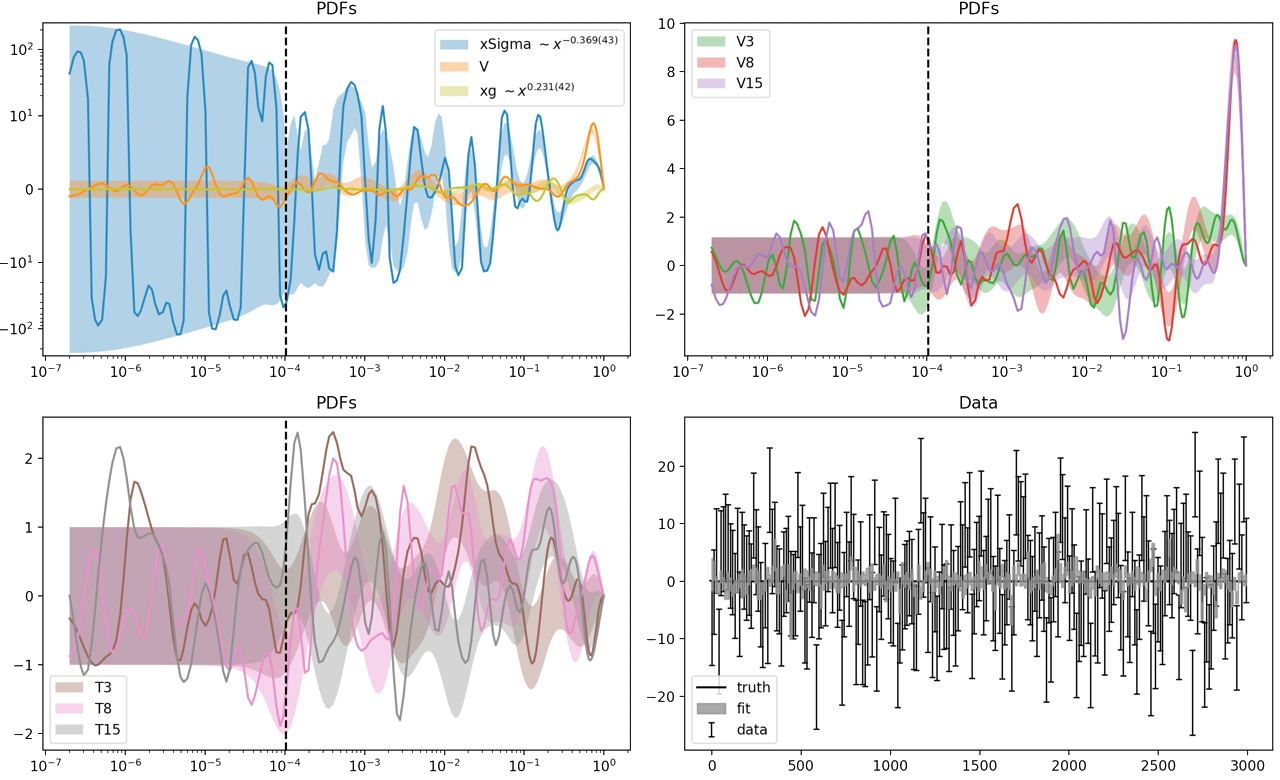
\includegraphics[width=\textwidth]{ch-gp/fit-pdf-new}
	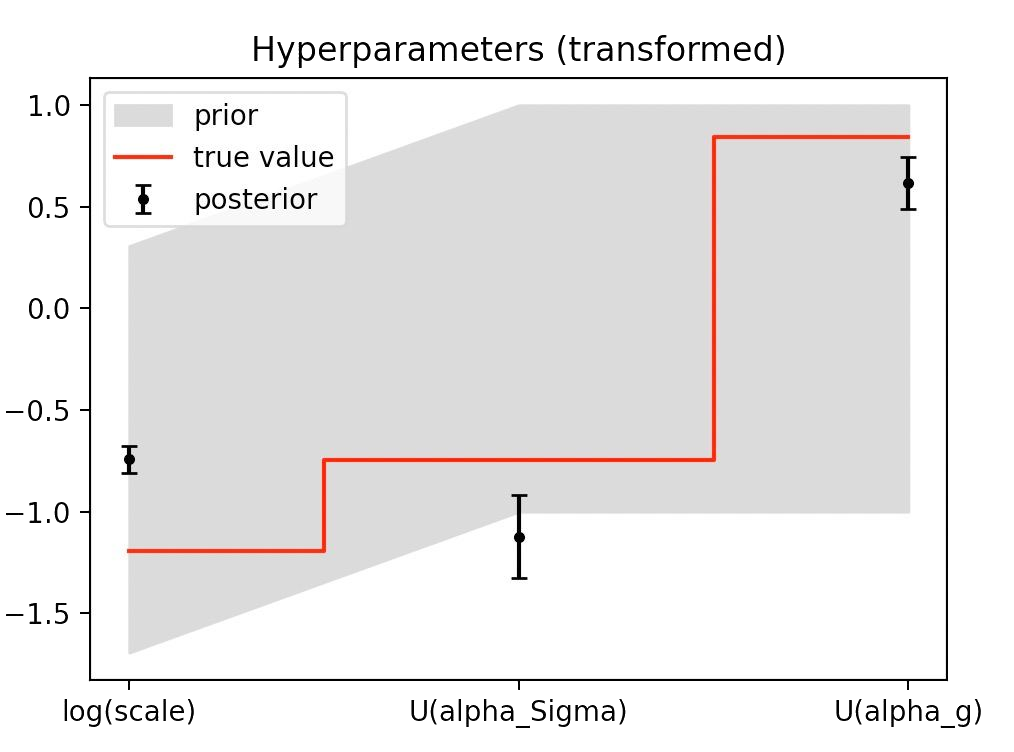
\includegraphics[width=0.55\textwidth]{ch-gp/fit-hyper-new}
  \caption{
    Current \lsqfitgp results on fake data.
    The lines are the underlying (fake) PDFs used to generate the fake data,
    while the bands are the $\pm 1\sigma$ intervals of the posterior.
    The vertical dashed lines mark the start of the $x$ values that are linked to the data. 
    The lower plot shows the inference over the hyperparameters, with the gray
    band representing the $\pm 1\sigma$ intervals of the prior.
  }
	\label{fig:gp/mcpdf}
\end{figure}
